\documentclass[aspectratio=169]{beamer}

\usetheme{Madrid}
\usecolortheme{default}

\usepackage[utf8]{inputenc}
\usepackage[T1]{fontenc}
\usepackage[brazil]{babel}
\usepackage{graphicx}
\usepackage{hyperref}
\usepackage{xcolor}
\usepackage{booktabs}
\usepackage{listings}

\definecolor{oceanblue}{RGB}{0,74,119}
\definecolor{oceanlight}{RGB}{219,238,244}
\definecolor{oceangreen}{RGB}{0,120,110}

\setbeamercolor{structure}{fg=oceanblue}
\setbeamercolor{frametitle}{fg=white,bg=oceanblue}
\setbeamercolor{title}{fg=white,bg=oceanblue}
\setbeamercolor{block title}{fg=white,bg=oceangreen}
\setbeamercolor{block body}{bg=oceanlight}

\lstset{
  basicstyle=\ttfamily\small,
  breaklines=true,
  frame=single,
  backgroundcolor=\color{gray!8}
}

\IfFileExists{curso-beamer.sty}{\usepackage{curso-beamer}}{}


\title[Desafios dos Dados N-Dimensionais]{Aula 2 --- Desafios dos Dados N-Dimensionais}
\subtitle{Da Ciência Tradicional ao Big Data\\
Novos Formatos e Fluxos para Dados Oceanográficos}
\author{Tobias Ferreira}
\institute{Instituto Nacional de Pesquisas Oceânicas (INPO)}
\date{01/09/2026}

\begin{document}

% ------------------------------------------------
\begin{frame}[plain,noframenumbering]
  \titlepage
\end{frame}

% ------------------------------------------------
\begin{frame}{Aula Anterior}
\Large
Na aula anterior vimos \textbf{formatos, metadados e padrões}.

\vspace{0.4cm}

Agora vamos olhar para o problema que motiva grande parte dos fluxos cloud-native:

\vspace{0.4cm}

\begin{block}{Pergunta central}
O que acontece quando nossos dados N-dimensionais deixam de ter alguns megabytes e passam a ocupar gigabytes, terabytes ou petabytes?
\end{block}
\end{frame}

% ------------------------------------------------
\begin{frame}{Objetivos da aula}
Ao final desta aula, você deverá conseguir:

\begin{itemize}
  \item descrever como NetCDF, GRIB e HDF5 organizam dados N-dimensionais;
  \item explicar por que os volumes de dados ambientais cresceram tanto nas últimas décadas;
  \item reconhecer limitações práticas ao abrir, mover e compartilhar arquivos grandes;
  \item explicar por que o acesso parcial é preferível ao download completo;
  \item relacionar chunking, memória, paralelismo e escalabilidade;
  \item usar xarray para inspecionar a estrutura de arquivos NetCDF e GRIB.
\end{itemize}
\end{frame}

% ------------------------------------------------
\begin{frame}{Perguntas que vamos responder}
\Large
\begin{itemize}
  \item Como NetCDF, GRIB e HDF5 representam grandes arrays?
  \item Por que os datasets cresceram tanto?
  \item O que acontece quando abrimos esses arquivos com xarray?
  \item Por que baixar o arquivo inteiro nem sempre faz sentido?
  \item Como chunking e acesso parcial ajudam?
  \item Onde formatos tradicionais começam a encontrar limites?
\end{itemize}
\end{frame}

% ------------------------------------------------
\begin{frame}{Dados ambientais são naturalmente N-dimensionais}
\begin{columns}
\column{0.48\textwidth}

Uma variável pode depender de várias dimensões:

\begin{itemize}
  \item longitude;
  \item latitude;
  \item altura ou profundidade;
  \item tempo;
  \item membro de ensemble;
  \item tempo de previsão;
  \item variável ou cenário.
\end{itemize}

\vspace{0.2cm}

\begin{block}{Exemplo}
\[
T = T(x,y,z,t,m)
\]
\end{block}

\column{0.52\textwidth}
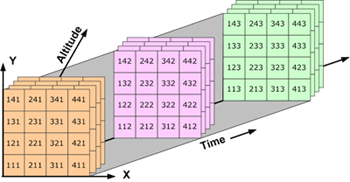
\includegraphics[width=\textwidth]{../episodes/fig/ndimensional.png}

\end{columns}
\end{frame}

% ------------------------------------------------
\begin{frame}{Por que isso se torna difícil?}
\begin{columns}
\column{0.33\textwidth}
\begin{block}{Mais dimensões}
Mais combinações possíveis de índices e subconjuntos.
\end{block}

\column{0.33\textwidth}
\begin{block}{Mais resolução}
Muito mais células para cada instante.
\end{block}

\column{0.33\textwidth}
\begin{block}{Mais tempo}
Arquivos e coleções crescem continuamente.
\end{block}
\end{columns}

\vspace{0.6cm}

\Large
\centering
\textbf{O desafio não é apenas armazenar os dados, mas encontrá-los, movê-los e acessar somente o que precisamos.}
\end{frame}

% ------------------------------------------------
\begin{frame}{NetCDF: arrays auto-descritivos}
\begin{itemize}
  \item Criado para dados científicos orientados a arrays.
  \item Armazena \textbf{variáveis}, \textbf{dimensões} e \textbf{atributos} no mesmo container.
  \item Permite que ferramentas descubram a estrutura do dataset durante a leitura.
  \item NetCDF-3 usa uma organização mais simples e contígua.
  \item NetCDF-4 utiliza HDF5 como camada de armazenamento e suporta grupos, grandes arrays e estruturas mais complexas.
\end{itemize}

\vspace{0.35cm}

\begin{block}{Visão do usuário}
Uma variável pode aparecer como \texttt{sst(time, latitude, longitude)} ou
\texttt{temperature(time, depth, latitude, longitude)}.
\end{block}
\end{frame}

% ------------------------------------------------
\begin{frame}{GRIB: compacto e orientado à operação}
\begin{itemize}
  \item Formato da WMO para transmissão e armazenamento eficiente de campos meteorológicos em grade.
  \item Organizado como uma sequência de \textbf{mensagens}.
  \item Cada mensagem contém um campo e metadados codificados.
  \item Usa tabelas da WMO para parâmetros, níveis e outros descritores.
  \item GRIB2 ampliou metadados, compressão e representação de valores ausentes.
\end{itemize}

\vspace{0.35cm}

\begin{block}{Vantagem e desafio}
É excelente para fluxos operacionais, mas um arquivo heterogêneo pode precisar ser filtrado ou reorganizado antes de parecer um único array N-dimensional.
\end{block}
\end{frame}

% ------------------------------------------------
\begin{frame}{HDF5: container hierárquico de alto desempenho}
\begin{itemize}
  \item Formato geral para datasets grandes e complexos.
  \item Organiza dados em \textbf{grupos}, \textbf{datasets} e \textbf{atributos}.
  \item Muito usado em sensoriamento remoto e produtos de observação da Terra.
  \item É a camada de armazenamento utilizada pelo NetCDF-4.
\end{itemize}

\vspace{0.4cm}

\begin{block}{Importante}
Quando usamos NetCDF-4, normalmente interagimos com o modelo NetCDF e não com os detalhes de baixo nível do HDF5.
\end{block}
\end{frame}

% ------------------------------------------------
\begin{frame}{Trinta anos de crescimento dos dados}
\begin{columns}
\column{0.45\textwidth}

Os volumes cresceram por causa de:

\begin{itemize}
  \item maior resolução espacial;
  \item maior resolução temporal;
  \item mais níveis verticais;
  \item arquivos históricos mais longos;
  \item ensembles de previsão e clima.
\end{itemize}

\vspace{0.15cm}

Coleções que antes ocupavam MB hoje podem alcançar TB ou PB.

\column{0.55\textwidth}
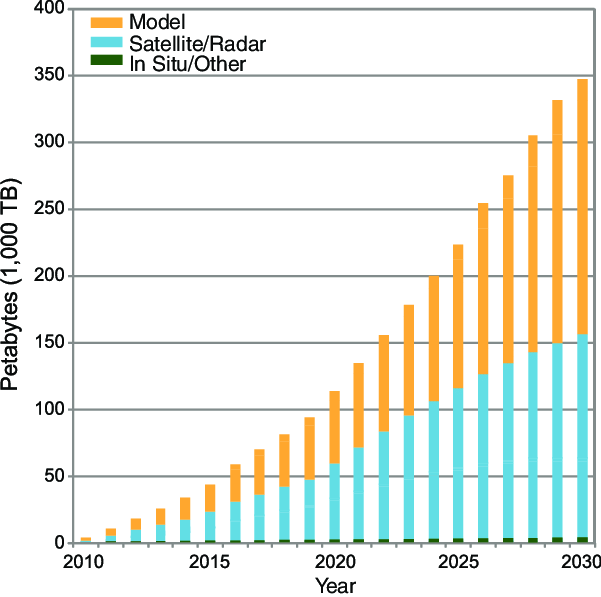
\includegraphics[height=6.5cm]{../episodes/fig/data_size_trends.png}

{\tiny Baseado em Overpeck et al. (2011).}
\end{columns}
\end{frame}


% ------------------------------------------------
\begin{frame}{O problema em escala real}
\scriptsize
\begin{table}
\centering
\renewcommand{\arraystretch}{1.10}
\begin{tabular}{>{\bfseries}p{0.20\textwidth} p{0.36\textwidth} p{0.15\textwidth} p{0.18\textwidth}}
\toprule
Dataset & Área / aplicação & Nº de arquivos & Tamanho \\
\midrule
CHESS-SCAPE & Projeções climáticas britânicas a 1 km, 1980--2080 & $\approx$387.840 & $\approx$11 TB \\
NOC NEMO NPD & Simulações oceânicas globais NEMO em diferentes resoluções & não consolidado & $\approx$71 TB \\
CMIP6 / ESGF & Modelos climáticos globais e experimentos acoplados & dezenas de milhões & $\approx$21 PB na agregação citada \\
ERA5 -- superfície & Reanálise atmosférica e de superfície do ECMWF & $\approx$5,31 milhões & $\approx$6 TB \\
ERA5 completo & Reanálise global horária & sem contagem única & ordem de PB \\
\bottomrule
\end{tabular}
\end{table}

\vspace{0.25cm}
\begin{block}{Mensagem}
O desafio deixa de ser apenas ``abrir um arquivo'' e passa a envolver arquitetura de acesso, organização, computação e compartilhamento.
\end{block}
\end{frame}


% ------------------------------------------------
\begin{frame}{Um pequeno aumento pode virar um grande problema}
Suponha uma grade com $N_x \times N_y$ pontos.

\vspace{0.4cm}

Se dobrarmos a resolução em cada direção horizontal:

\[
(2N_x)(2N_y) = 4N_xN_y
\]

\vspace{0.3cm}

Ou seja, temos aproximadamente \textbf{quatro vezes mais células} por instante.

\vspace{0.4cm}

Agora combine isso com:

\begin{itemize}
  \item mais níveis de profundidade;
  \item saídas a cada 10 minutos;
  \item 30 anos de dados;
  \item dezenas de membros de ensemble.
\end{itemize}
\end{frame}

% ------------------------------------------------
\begin{frame}{Como trabalhamos com esses dados hoje?}
Em muitos fluxos científicos:

\begin{itemize}
  \item NetCDF é usado para análise e arquivamento;
  \item GRIB é usado para produtos operacionais e intercâmbio;
  \item xarray apresenta os dois como datasets N-dimensionais rotulados;
  \item arquivos ficam em discos locais, servidores compartilhados ou HPC;
  \item usuários baixam ou copiam dados antes de executar a análise.
\end{itemize}

\vspace{0.4cm}

\begin{block}{Ponto importante}
A interface de alto nível pode parecer simples, mas o desempenho depende da organização física, do tamanho dos arquivos, do hardware e do padrão de acesso.
\end{block}
\end{frame}

% ------------------------------------------------
\begin{frame}[fragile]{Exercício 1 --- Inspecionando um NetCDF}
\textbf{Dataset:} ERA5 SST, com campos 2D de temperatura da superfície do mar.

\vspace{0.25cm}

\begin{lstlisting}[language=Python]
import xarray as xr

base_path = (
    "/gws/ssde/j25b/atlantis_vis/"
    "cloud-native-geoscience-course/"
)

ds = xr.open_dataset(
    f"{base_path}data/era5_sst/ocean_temperature.nc"
)

print(ds)
print(ds.dims)
print(ds.coords)
print(ds.attrs)
\end{lstlisting}
\end{frame}

% ------------------------------------------------
\begin{frame}{Exercício 1 --- O que observar?}
\begin{itemize}
  \item Quais dimensões existem?
  \item Como tempo, latitude e longitude aparecem?
  \item Quais coordenadas estão associadas às dimensões?
  \item Que atributos descrevem a origem e as convenções do arquivo?
  \item Como a estrutura mudaria se adicionássemos profundidade ou ensemble?
\end{itemize}

\end{frame}

% ------------------------------------------------
\begin{frame}[fragile]{Exercício 2 --- Comparando NetCDF e GRIB}
\begin{lstlisting}[language=Python]
ds_nc = xr.open_dataset(
    f"{base_path}data/era5_sst/ocean_temperature.nc"
)

ds_grib = xr.open_dataset(
    f"{base_path}data/era5_sst/ocean_temperature.grib",
    engine="cfgrib",
)

print(ds_nc)
print(ds_grib)
print(ds_grib.data_vars)
\end{lstlisting}

\vspace{0.2cm}

\textbf{Pergunta:} os dois formatos parecem muito diferentes quando vistos pelo xarray?
\end{frame}

% ------------------------------------------------
\begin{frame}{NetCDF e GRIB vistos pelo xarray}
No exemplo da aula, ambos representam praticamente o mesmo campo científico:

\begin{itemize}
  \item mesma grade espacial;
  \item 120 passos de tempo;
  \item uma variável principal: \texttt{sst}.
\end{itemize}

\vspace{0.3cm}

Mas existem diferenças:

\begin{itemize}
  \item o NetCDF usa uma representação CF mais direta;
  \item o GRIB preserva coordenadas auxiliares e metadados específicos do formato;
  \item o GRIB é internamente baseado em mensagens, mesmo que o xarray apresente uma visão N-dimensional.
\end{itemize}
\end{frame}

% ------------------------------------------------
\begin{frame}{Exercício 3 --- Pensando em escala}
Imagine que:

\begin{itemize}
  \item a resolução horizontal dobra em latitude e longitude;
  \item a frequência muda de 1 hora para 10 minutos;
  \item o período aumenta para 30 anos;
  \item vários grupos precisam analisar o mesmo dataset.
\end{itemize}

\vspace{0.4cm}

Discuta:

\begin{enumerate}
  \item Como as dimensões e o número de células mudam?
  \item Como o tamanho do arquivo e do arquivo histórico mudam?
  \item O que acontece com memória, leitura e tempo de processamento?
  \item Como você compartilharia esses dados?
\end{enumerate}
\end{frame}

% ------------------------------------------------
\begin{frame}{O modelo tradicional: baixar primeiro}
\Large
\centering

Publicar NetCDF/GRIB em portal, FTP ou HTTP

\vspace{0.25cm}
$\Downarrow$

Baixar o arquivo completo

\vspace{0.25cm}
$\Downarrow$

Salvar no computador ou servidor

\vspace{0.25cm}
$\Downarrow$

Abrir e extrair o subconjunto necessário

\vspace{0.45cm}

\textbf{Funciona bem para dados pequenos. Escala mal para grandes arquivos históricos.}
\end{frame}

% ------------------------------------------------
\begin{frame}{Por que baixar tudo é ineficiente?}
\begin{itemize}
  \item O usuário pode querer apenas uma variável.
  \item Talvez precise de uma pequena região geográfica.
  \item Talvez precise de alguns dias de uma série de 30 anos.
  \item O download completo consome rede, tempo e armazenamento.
  \item Vários usuários criam cópias duplicadas do mesmo dataset.
  \item Cópias locais podem terminar em versões diferentes do mesmo dado.
\end{itemize}

\vspace{0.3cm}

\begin{block}{Objetivo}
Levar a computação até o dado, ou permitir que o usuário leia apenas os bytes necessários.
\end{block}
\end{frame}

% ------------------------------------------------
\begin{frame}{Acesso parcial e subsetting}
Em vez de transferir o arquivo inteiro, queremos solicitar:

\begin{itemize}
  \item uma caixa espacial;
  \item um intervalo de tempo;
  \item uma profundidade;
  \item uma variável;
  \item alguns membros de ensemble.
\end{itemize}

\vspace{0.4cm}

Protocolos como \textbf{OPeNDAP} e APIs modernas já permitem subsetting no servidor.

\vspace{0.3cm}

\begin{block}{Limitação}
Isso reduz transferência, mas exige infraestrutura de servidor e o desempenho ainda depende da carga do serviço e da rede.
\end{block}
\end{frame}

% ------------------------------------------------
\begin{frame}{Chunking: dividir para acessar melhor}
\Large
Chunking divide um array grande em blocos menores.

\vspace{0.4cm}

\begin{columns}
\column{0.5\textwidth}
\begin{block}{Array monolítico}
Ler uma pequena região pode envolver grandes operações de I/O.
\end{block}

\column{0.5\textwidth}
\begin{block}{Array dividido em chunks}
Podemos buscar somente os blocos que intersectam o subconjunto desejado.
\end{block}
\end{columns}

\vspace{0.5cm}

\centering
\textbf{Chunking conecta organização física, memória, paralelismo e desempenho.}
\end{frame}

% ------------------------------------------------
\begin{frame}{POSIX versus object storage}
\begin{columns}
\column{0.5\textwidth}
\textbf{POSIX / filesystem tradicional}

\begin{itemize}
  \item arquivos e diretórios;
  \item disco local ou filesystem montado;
  \item comum em HPC e servidores;
  \item operações tradicionais de arquivo.
\end{itemize}

\column{0.5\textwidth}
\textbf{Object storage}

\begin{itemize}
  \item dados armazenados como objetos;
  \item acesso por APIs;
  \item escala horizontal;
  \item adequado para grandes arquivos históricos compartilhados;
  \item comum em infraestrutura cloud.
\end{itemize}
\end{columns}

\vspace{0.3cm}

\begin{block}{Problema de compatibilidade}
NetCDF/HDF5 clássicos foram desenvolvidos principalmente para sistemas de arquivos POSIX, não para acesso direto e altamente paralelo a object storage.
\end{block}
\end{frame}

% ------------------------------------------------
\begin{frame}{Xarray é lazy, mas isso não resolve tudo}
\begin{itemize}
  \item Ao abrir um NetCDF, xarray pode inspecionar metadados sem carregar todos os valores.
  \item Isso é chamado de \textbf{lazy loading}.
  \item Porém, quando uma operação precisa dos valores, partes grandes do arquivo podem ter de ser lidas.
  \item Se o dataset não estiver organizado de acordo com o padrão de acesso, a leitura pode continuar cara.
\end{itemize}

\vspace{0.4cm}

\begin{block}{Consequência}
A interface Python pode ser simples, mas a organização dos dados continua determinando o custo real da análise.
\end{block}
\end{frame}

% ------------------------------------------------
\begin{frame}{Formato, escala e acesso}
\begin{columns}
\column{0.33\textwidth}
\begin{block}{Formato}
Como os arrays e metadados são organizados?
\end{block}

\column{0.33\textwidth}
\begin{block}{Escala}
Quantos bytes, arquivos, dimensões e usuários existem?
\end{block}

\column{0.33\textwidth}
\begin{block}{Acesso}
Quais partes do dataset realmente precisamos ler?
\end{block}
\end{columns}

\vspace{0.7cm}

\Large
\centering
\textbf{Esses três fatores precisam ser considerados juntos.}
\end{frame}

% ------------------------------------------------
\begin{frame}{Por que isso nos leva ao cloud-native?}
\begin{itemize}
  \item Grandes coleções não devem depender de downloads completos.
  \item Precisamos de acesso parcial eficiente.
  \item O armazenamento precisa escalar sem multiplicar cópias.
  \item O processamento precisa explorar paralelismo.
  \item A organização física deve combinar com o padrão de acesso.
\end{itemize}

\vspace{0.4cm}

\begin{block}{Próximo passo}
Nas próximas aulas veremos como formatos cloud-native, especialmente \textbf{Zarr}, combinam chunks, object storage e ferramentas como xarray e Dask para atacar esses problemas.
\end{block}
\end{frame}

% ------------------------------------------------
\begin{frame}{Resumo}
\begin{itemize}
  \item Dados oceanográficos e meteorológicos são naturalmente N-dimensionais.
  \item NetCDF, GRIB e HDF5 continuam fundamentais para a ciência e a operação.
  \item Resolução, frequência, arquivos históricos e ensembles multiplicaram o volume dos dados.
  \item O fluxo ``baixar tudo e analisar depois'' deixa de escalar.
  \item Acesso parcial, chunking e processamento paralelo tornam-se essenciais.
  \item Formato, escala e padrão de acesso precisam ser pensados em conjunto.
  \item Esses desafios motivam os formatos e arquiteturas cloud-native.
\end{itemize}
\end{frame}

\end{document}
